\documentclass[journal,12pt,twocolumn]{IEEEtran}

\usepackage{setspace}
\usepackage{gensymb}

\singlespacing


\usepackage[cmex10]{amsmath}

\usepackage{amsthm}

\usepackage{mathrsfs}
\usepackage{txfonts}
\usepackage{stfloats}
\usepackage{bm}
\usepackage{cite}
\usepackage{cases}
\usepackage{subfig}

\usepackage{longtable}
\usepackage{multirow}

\usepackage{enumitem}
\usepackage{mathtools}
\usepackage{steinmetz}
\usepackage{tikz}
\usepackage{circuitikz}
\usepackage{verbatim}
\usepackage{tfrupee}
\usepackage[breaklinks=true]{hyperref}
\usepackage{graphicx}
\usepackage{tkz-euclide}

\usetikzlibrary{calc,math}
\usepackage{listings}
    \usepackage{color}                                            %%
    \usepackage{array}                                            %%
    \usepackage{longtable}                                        %%
    \usepackage{calc}                                             %%
    \usepackage{multirow}                                         %%
    \usepackage{hhline}                                           %%
    \usepackage{ifthen}                                           %%
    \usepackage{lscape}     
\usepackage{multicol}
\usepackage{chngcntr}

\DeclareMathOperator*{\Res}{Res}

\renewcommand\thesection{\arabic{section}}
\renewcommand\thesubsection{\thesection.\arabic{subsection}}
\renewcommand\thesubsubsection{\thesubsection.\arabic{subsubsection}}

\renewcommand\thesectiondis{\arabic{section}}
\renewcommand\thesubsectiondis{\thesectiondis.\arabic{subsection}}
\renewcommand\thesubsubsectiondis{\thesubsectiondis.\arabic{subsubsection}}


\hyphenation{op-tical net-works semi-conduc-tor}
\def\inputGnumericTable{}                                 %%

\lstset{
%language=C,
frame=single, 
breaklines=true,
columns=fullflexible
}
\begin{document}


\newtheorem{theorem}{Theorem}[section]
\newtheorem{problem}{Problem}
\newtheorem{proposition}{Proposition}[section]
\newtheorem{lemma}{Lemma}[section]
\newtheorem{corollary}[theorem]{Corollary}
\newtheorem{example}{Example}[section]
\newtheorem{definition}[problem]{Definition}

\newcommand{\BEQA}{\begin{eqnarray}}
\newcommand{\EEQA}{\end{eqnarray}}
\newcommand{\define}{\stackrel{\triangle}{=}}
\bibliographystyle{IEEEtran}
\providecommand{\mbf}{\mathbf}
\providecommand{\pr}[1]{\ensuremath{\Pr\left(#1\right)}}
\providecommand{\qfunc}[1]{\ensuremath{Q\left(#1\right)}}
\providecommand{\sbrak}[1]{\ensuremath{{}\left[#1\right]}}
\providecommand{\lsbrak}[1]{\ensuremath{{}\left[#1\right.}}
\providecommand{\rsbrak}[1]{\ensuremath{{}\left.#1\right]}}
\providecommand{\brak}[1]{\ensuremath{\left(#1\right)}}
\providecommand{\lbrak}[1]{\ensuremath{\left(#1\right.}}
\providecommand{\rbrak}[1]{\ensuremath{\left.#1\right)}}
\providecommand{\cbrak}[1]{\ensuremath{\left\{#1\right\}}}
\providecommand{\lcbrak}[1]{\ensuremath{\left\{#1\right.}}
\providecommand{\rcbrak}[1]{\ensuremath{\left.#1\right\}}}
\theoremstyle{remark}
\newtheorem{rem}{Remark}
\newcommand{\sgn}{\mathop{\mathrm{sgn}}}
\providecommand{\abs}[1]{\left\vert#1\right\vert}
\providecommand{\res}[1]{\Res\displaylimits_{#1}} 
\providecommand{\norm}[1]{\left\lVert#1\right\rVert}
%\providecommand{\norm}[1]{\lVert#1\rVert}
\providecommand{\mtx}[1]{\mathbf{#1}}
\providecommand{\mean}[1]{E\left[ #1 \right]}
\providecommand{\fourier}{\overset{\mathcal{F}}{ \rightleftharpoons}}
%\providecommand{\hilbert}{\overset{\mathcal{H}}{ \rightleftharpoons}}
\providecommand{\system}{\overset{\mathcal{H}}{ \longleftrightarrow}}
	%\newcommand{\solution}[2]{\textbf{Solution:}{#1}}
\newcommand{\solution}{\noindent \textbf{Solution: }}
\newcommand{\cosec}{\,\text{cosec}\,}
\providecommand{\dec}[2]{\ensuremath{\overset{#1}{\underset{#2}{\gtrless}}}}
\newcommand{\myvec}[1]{\ensuremath{\begin{pmatrix}#1\end{pmatrix}}}
\newcommand{\mydet}[1]{\ensuremath{\begin{vmatrix}#1\end{vmatrix}}}
\numberwithin{equation}{subsection}
\makeatletter
\@addtoreset{figure}{problem}
\makeatother
\let\StandardTheFigure\thefigure
\let\vec\mathbf
\renewcommand{\thefigure}{\theproblem}
\def\putbox#1#2#3{\makebox[0in][l]{\makebox[#1][l]{}\raisebox{\baselineskip}[0in][0in]{\raisebox{#2}[0in][0in]{#3}}}}
     \def\rightbox#1{\makebox[0in][r]{#1}}
     \def\centbox#1{\makebox[0in]{#1}}
     \def\topbox#1{\raisebox{-\baselineskip}[0in][0in]{#1}}
     \def\midbox#1{\raisebox{-0.5\baselineskip}[0in][0in]{#1}}
\vspace{3cm}
\title{EE5609 Matrix Theory}
\author{Kranthi Kumar P}
\date{September 2020}
\maketitle
\newpage
\bigskip
\renewcommand{\thefigure}{\theenumi}
\renewcommand{\thetable}{\theenumi}
Download the python code for circle from 
\begin{lstlisting}
https://github.com/kranthiakssy/AI20RESCH14002_PhD_IITH/tree/master/EE5609_Matrix_Theory/Assignment-6
\end{lstlisting}

Download the latex-file codes from 
%
\begin{lstlisting}
https://github.com/kranthiakssy/AI20RESCH14002_PhD_IITH/tree/master/EE5609_Matrix_Theory/Assignment-6
\end{lstlisting}
\section*{Assignment-6\\ramsey}
\subsection*{Problem:}
Affine Transformation (3.4.8):\\
Show that, by changing the origin, the equation
\begin{align}
2\vec{x}^T\vec{x}+\myvec{7&5}\vec{x}-13=0
\label{eq:a0}
\end{align}
can be transformed to
\begin{align}
8\vec{x}^T\vec{x}=89
\label{eq:a1}
\end{align}
\subsection*{Solution:}
Eq \eqref{eq:a0} cab be written as
\begin{align}
\vec{x}^T\vec{x}+\myvec{\frac{7}{2}&\frac{5}{2}}\vec{x}-\frac{13}{2}=0\\
\implies \vec{x}^T\vec{x}+2\myvec{\frac{7}{4}&\frac{5}{4}}\vec{x}-\frac{13}{2}=0
\label{eq:a2}
\end{align}
The above eq \eqref{eq:a2} cab be compared with the circle equation gives as
\begin{align}
\vec{x}^T\vec{x}+2\vec{u}^T\vec{x}+f=0
\label{eq:a3}
\end{align}
\begin{figure}[!ht]
	\centering
	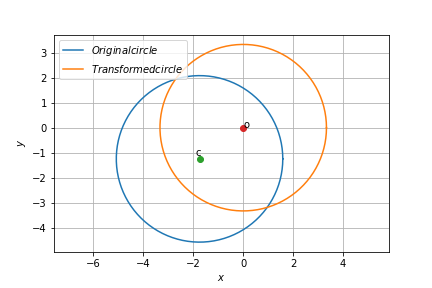
\includegraphics[width=\columnwidth]{circle.png}
	\caption{Figure depicting transformation of circle}
	\label{myfig}
\end{figure}
then
\begin{align}
\vec{u} = \myvec{\frac{7}{4}\\\frac{5}{4}}\\
\label{eq:a4}
\implies centre, \vec{c} = \myvec{\frac{-7}{4}\\\frac{-5}{4}}\\
\norm{u}^2 - r^2 = f\\
\implies r^2 = \norm{u}^2 - f\\
\implies r^2 = \left(\frac{7}{4}\right)^2+\left(\frac{5}{4}\right)^2+\frac{13}{2}\\
\implies radius, r = \sqrt{\frac{89}{8}}
\end{align}
The eq \eqref{eq:a1} can be written by changing the origin as
\begin{align}
\vec{(x+c)}^T\vec{(x+c)} = \frac{89}{8}\\
\implies \vec{x}^T\vec{x}+\vec{x}^T\vec{c}+\vec{c}^T\vec{x}+\vec{c}^T\vec{c} = \frac{89}{8}
\label{eq:a5}
\end{align}
We know that
\begin{align}
\vec{x}^T\vec{c} = \vec{c}^T\vec{x}
\label{eq:a6}
\end{align}
by substituting \eqref{eq:a6} in \eqref{eq:a5}
\begin{align}
\vec{x}^T\vec{x}+2\vec{c}^T\vec{x}+\vec{c}^T\vec{c} = \frac{89}{8}
\label{eq:a7}
\end{align}
substituting the orgin of \eqref{eq:a0} in above eq \eqref{eq:a7}
\begin{align}
\vec{x}^T\vec{x}+2\myvec{\frac{7}{4}&\frac{5}{4}}\vec{x}+\myvec{\frac{-7}{4}&\frac{-5}{4}}\myvec{\frac{-7}{4}\\\frac{-5}{4}} = \frac{89}{8}\\
\implies \vec{x}^T\vec{x}+\myvec{\frac{7}{2}&\frac{5}{2}}\vec{x}+\frac{74}{16}-\frac{89}{8} = 0\\
\implies \vec{x}^T\vec{x}+\myvec{\frac{7}{2}&\frac{5}{2}}\vec{x}-\frac{13}{2} = 0\\
\implies 2\vec{x}^T\vec{x}+\myvec{7&5}\vec{x}-13 = 0
\end{align}
$\therefore$ It is proved that by changing the origin in \eqref{eq:a1} we obtained \eqref{eq:a0}.
\end{document}